\chapter{Задача о сдавливании сферического идеально жесткопластического слоя}\label{ch:ch3}
На основе анализа классической задачи Прандтля \autocite{Prandtl:1948} получены значительные результаты связанные с теорией течение по поверхностям, которые имеют широкое применение для решения технологических задач. Одним из обобщений данной задачи является случай осесимметричного меридионального течения со стоком между двумя концентрическими шероховатыми сферами \autocite{Georgievsky:2011}.
Решение данной задачи применимо в различных технологиях изготовления тонких сферических тел, например в штамповке взрывом.
% \fixme{Сформулировать мысль про применение в каком-нибудь процессе формообразования, например в штамповке взрывом.} 
В данной постановке задачи исследуется влияние динамических эффектов в процессе формирования изделия методом прессования. Материалы главы содержатся в публикации \autocite{Shabaykin:2020a}.

\section{Постановка задачи и асимптотические разложения}\label{sec:ch3/sec1}

Пренебрегая начальными упругими деформациями, вязкостью и незначительным упрочнением, материал, имеющий плотность $\varrho$, полагается несжимаемым идеально жесткопластическим, удовлетворяющим тензорно линейным определяющим соотношениям и скалярному определяющему соотношению -- квадратичному критерию Мизеса-Генки $\sigma_{u} = \sigma_{s}$, где $\sigma_{u} = \sqrt{\utilde{s} : \utilde{s}}$ -- интенсивность напряжения, $\utilde{s}$ -- девиатор напряжения, $\sigma_{s}$ -- предел текучести.

Пусть течение происходит в области
\begin{equation}
  \Omega_{t} = \{0 \le r \le R(t)+ h(t), 0 \le \theta < \pi, 0 \le \phi < 2\pi\},
\end{equation}
с границей $\partial\Omega = \Gamma = \Gamma_{1} \cup \Gamma_{2}$, причем $h(t) \ll R(t)$ для любого $t \ge 0$.

Внешняя сфера неподвижна, а внутренняя радиально расширяется с постоянной скоростью, выдавливая материал через сток $\theta=\pi$.

\begin{figure}[ht]
  \centerfloat{
    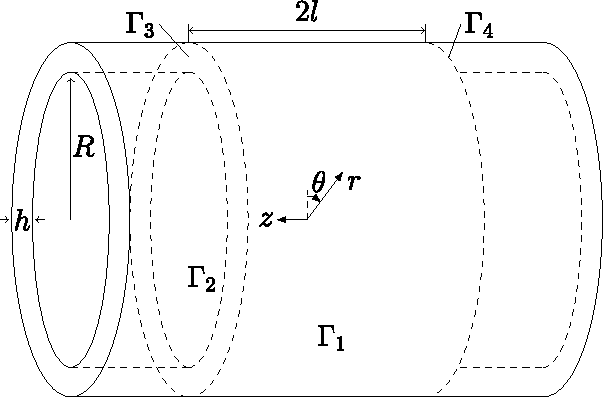
\includegraphics[width=0.4\linewidth]{./ch3/layer}
  }
  \caption{Представление сферического слоя}
  \label{fig:ch3/layer/circle}
\end{figure}
Скорость расширения внутренней сферы обозначим $V$, поэтому кинематическое условие непротекания сквозь границы $\Gamma_{1}$ и $\Gamma_{2}$ имеет вид
\begin{equation}
  \label{eq:ch3/sec1/boundary/kinematic}
  v_{r}\lvert_{r=R} = V, \quad v_{r}\lvert_{r=R + h} = 0
\end{equation}
Касательная составляющая скорости (в данном случае $v_{\theta}$) на указанных границах идеальной среды, как известно, не задаётся.

В некоторый момент времени $0 < t <  h_{0}/V = t_*$, где $t_*$ -- момент схлопывания слоя, относительно шести функций -- независимых компонент девиатора напряжений $s_{rr}$, $s_{r\theta}$ и $s_{\theta\theta}$, давления $p$ и компонент скорости $v_{r}$ и $v_{\theta}$ -- должна выполнятся замкнутая система уравнений динамической теории идеальной пластичности для цилиндрических координат:
\begin{gather}
  \label{eqs:ch3/sec1/general/motion:1}
  \begin{multlined}
    -p_{,r}+s_{rr,r}+\frac{1}{r}\left(s_{r\theta,\theta}+3s_{rr}+s_{r\theta}\cot{\left(\theta\right)}\right) \unl{=}
    \varrho \left(v_{r;t}+v_{r} v_{r,r} + \frac{1}{r}v_{\theta} v_{r,\theta} - \frac{1}{r} v_{\theta}^2 \right)
  \end{multlined}
  \\
  \label{eqs:ch3/sec1/general/motion:2}
  \begin{multlined}
    -\frac{1}{r} p_{,\theta}+s_{r\theta,r}+\frac{1}{r}\left(s_{\theta\theta,\theta}+3s_{r\theta}+\left(s_{rr}+2s_{\theta\theta}\right)\cot{\left(\theta\right)}\right) \unl{=}
    \varrho \left(v_{\theta;t}+v_{r} v_{\theta,r} + \frac{1}{r}v_{\theta} v_{\theta,\theta} - \frac{1}{r} v_{\theta} v_{r} \right)
  \end{multlined}
  \\
  \label{eqs:ch3/sec1/general/plasticity}
  s^2_{rr}+s^2_{\theta\theta}+s_{rr} s_{\theta\theta} + s^2_{r\theta}=\tau^2_{s}
  \\
  \label{eqs:ch3/sec1/general/coax:1}
  s_{rr} \left(v_{\theta,\theta} + v_{r}\right) / r = s_{\theta\theta} v_{r,r}
  \\
  \label{eqs:ch3/sec1/general/coax:2}
  s_{rr} \left(v_{\theta,r}+\left(v_{r,\theta}-v_{\theta}\right) / r\right) = 2 s_{r\theta} v_{r,r}
  \\
  \label{eqs:ch3/sec1/general/uncompress}
  v_{r,r}+\left(2v_{r}+v_{\theta,\theta}+v_{\theta}\cot{\left(\theta\right)}\right) / r = 0
\end{gather}

\expandafter\gdef\csname eqs:ch3/sec1/general\endcsname{eqs:ch3/sec1/general/motion:1,eqs:ch3/sec1/general/motion:2,eqs:ch3/sec1/general/plasticity,eqs:ch3/sec1/general/coax:1,eqs:ch3/sec1/general/coax:2,eqs:ch3/sec1/general/uncompress}
Кроме выполнения условия \cref{eq:ch3/sec1/boundary/kinematic} на жестких контактирующих поверхностях потербуем, что бы модуль касательного напряжения $s_{r\theta}$ достигал на границах $\Gamma_{1}$ и $\Gamma_{2}$ своего максимального значения:
\begin{equation}
  \label{eq:ch3/sec1/boundary/force}
  \lvert s_{r\theta}\lvert_{r=R} = \lvert s_{r\theta}\lvert_{r=R+h} = \mu(\theta) \tau_{s}, \quad 0 < \mu \le 1,
\end{equation}
где $\mu$ -- шероховатость пресса. Абсолютной шероховатости, или полному сцеплению пресса с материалом, соответствует значение $\mu = 1$.


Введем малый параметр $\alpha = \frac{h(t)}{R(t)} \ll 1$ и проведем разложение всех неизвестных величин, входящих в систему уравнений \cref{\csname eqs:ch3/sec1/general\endcsname}, в ряды по целым степеням параметра:
\begin{gather}
  \label{eqs:ch3/series/vt}
  v_{\theta}\left(r, \theta, t\right) = V \sum_{k=-N}^{\infty}{\alpha^{k} \; \uindex{v}{k}_{\theta}}, \quad N \ge 1
  \\
  \label{eqs:ch3/series/vr}
  v_{r}\left(r, \theta, t\right) = V \sum_{k=0}^{\infty}{\alpha^{k} \; \uindex{v}{k}_{r}}
  \\
  \label{eqs:ch3/series/sij}
  s_{ij}\left(r, \theta, t\right) = \tau_{s} \sum_{k=0}^{\infty}{\alpha^{k} \; \uindex{s}{k}_{ij}}, \quad (ij)\in\{rr, r\theta, \theta\theta\}
  \\
  \label{eqs:ch3/series/p}
  p\left(r, \theta, t \right) = \tau_{s} \sum_{k=-M}^{\infty}{\alpha^{k} \; \uindex{p}{k}}, \quad M \ge 1
\end{gather}

\expandafter\gdef\csname eqs:ch3/series\endcsname{eqs:ch3/series/vt,eqs:ch3/series/vr,eqs:ch3/series/sij,eqs:ch3/series/p}
Коэффициенты рядов \cref{\csname eqs:ch3/series\endcsname} -- безразмерны и являются функциями безразмерных координат $\rho, \theta, \tau$ :
\begin{equation}
  \label{eq:ch3/coordinates}
  \rho = \frac{r-R}{h}, \quad \tau = V \frac{t}{h}
\end{equation}
Наличие в \cref{\csname eqs:ch3/series\endcsname} членов $\alpha^{-n} \; \uindex{v}{-n}_{\theta}$ и $\alpha^{-m} \; \uindex{p}{-m}$ обусловлено стремлением $v_{r}$ и $p$ к бесконечности, при $\alpha\rightarrow 0$, что ясно из физических соображений.
Используя равенство $\dot{R}=-\dot{h}= V$ выразим малый параметр и координаты \cref{eq:ch3/coordinates} как эволюционные функции:
\begin{gather}
  \dot{\alpha} = \left(\frac{h}{R}\right)^. = \frac{\dot{h}R - h\dot{R}}{h^2} = -\frac{V}{h} \alpha \left(1+\alpha\right)
  \\
  \dot{\rho} = \left(\frac{r-R}{h}\right)^. = \frac{\dot{R} h - \left(r-R\right) \dot{h}}{h^2} = -\frac{V}{h}\left(1-\rho\right)
  \\
  \dot{\tau} = \left(V \frac{t}{h}\right)^. = V \frac{h - t\dot{h}}{h^2} = \frac{V}{h} \left(1+\tau\right)
\end{gather}
Подставляя выражения \cref{\csname eqs:ch3/series\endcsname} в систему \cref{\csname eqs:ch3/sec1/general\endcsname} и учитывая, что полная производная по времени представляется в виде
\begin{equation*}
  \uindex{v}{k}_{i;t} = \uindex{v}{k}_{i,\rho} \dot{\rho} + \uindex{v}{k}_{i,\tau} \dot{\tau}
\end{equation*}
получим следующую систему:
\begingroup
\allowdisplaybreaks
\begin{gather}
  \label{eqs:ch3/sec1/substituted/motion:1}
  \begin{multlined}
    -\!\!\!\!\sum_{k=-M}^{\infty}{\!\!\alpha^{k} \; \uindex{p}{k}_{,\rho}}{+}\sum_{k=0}^{\infty}{\alpha^{k} \; \uindex{s}{k}_{rr,\rho}}{+}
    \frac{\alpha}{1{+}\alpha\rho} \sum_{k=0}^{\infty}\alpha^{k} \left(\ \uindex{s}{k}_{r\theta,\theta} + 3\ \uindex{s}{k}_{rr} + \uindex{s}{k}_{r\theta}\cot{\left(\theta\right)}\right) \unl{=} \frac{\varrho V^2}{\tau_{s}}\left( \vphantom{\left(\sum_{k=-N}^{\infty}\right)^2}
    \sum_{k=0}^{\infty}\alpha^{k} \left(\;
    \left(1-\rho\right)\uindex{v}{k}_{r,\rho} + \uindex{v}{k}_{r,\theta} + \left(1+\tau\right)\uindex{v}{k}_{r,\tau} - \left(1+\alpha\right)\uindex{v}{k}_{r}
    \right) \unl[1]{+}
    \sum_{k=0}^{\infty}{\alpha^{k} \; \uindex{v}{k}_{r}} \sum_{k=0}^{\infty}{\alpha^{k} \; \uindex{v}{k}_{r,\rho}} {+} \frac{\alpha}{1{+}\alpha\rho} \left( \vphantom{\left(\sum_{k=-N}^{\infty}\right)^2}
    \sum_{k=-N}^{\infty}{\alpha^{k} \; \uindex{v}{k}_{\theta}} \sum_{k=0}^{\infty}{\alpha^{k} \; \uindex{v}{k}_{r,\theta}} \unl[2]{-}
    \left(\sum_{k=-N}^{\infty}{\alpha^{k} \; \uindex{v}{k}_{\theta}}\right)^2
    \right)
    \right)
  \end{multlined}
  \\
  \label{eqs:ch3/sec1/substituted/motion:2}
  \begin{multlined}
    -\frac{\alpha}{1+\alpha\rho}\sum_{k=-M}^{\infty}{\alpha^{k} \; \uindex{p}{k}_{,\theta}}+\sum_{k=0}^{\infty}{\alpha^{k} \; \uindex{s}{k}_{r\theta,\rho}}+
    \frac{\alpha}{1+\alpha\rho} \sum_{k=0}^{\infty}\alpha^{k} \left(\ \uindex{s}{k}_{\theta\theta,\theta} + 3\ \uindex{s}{k}_{r\theta} \unl[1]{+}
    \left(\ \uindex{s}{k}_{rr}+2\uindex{s}{k}_{\theta\theta}\right)\cot{\left(\theta\right)}\right) \unl{=}
    \frac{\varrho V^2}{\tau_{s}}\left(
    \sum_{k=-N}^{\infty}\alpha^{k} \left(\;
    \left(1-\rho\right)\uindex{v}{k}_{\theta,\rho} + \uindex{v}{k}_{\theta,\theta} + \left(1+\tau\right)\uindex{v}{k}_{\theta,\tau} - \left(1+\alpha\right)\uindex{v}{k}_{\theta}
    \right) \unl[1]{+}
    \sum_{k=0}^{\infty}{\alpha^{k} \; \uindex{v}{k}_{r}} \sum_{k=-N}^{\infty}{\alpha^{k} \; \uindex{v}{k}_{\theta,\rho}} {+} \frac{\alpha}{1{+}\alpha\rho} \left( \vphantom{\left(\sum_{k=-N}^{\infty}\right)^2}
    \sum_{k=-N}^{\infty}{\alpha^{k} \; \uindex{v}{k}_{\theta}} \sum_{k=0}^{\infty}{\alpha^{k} \; \uindex{v}{k}_{r,\theta}} \unl[2]{-}
    \sum_{k=-N}^{\infty}{\alpha^{k} \; \uindex{v}{k}_{\theta}} \sum_{k=0}^{\infty}{\alpha^{k} \; \uindex{v}{k}_{r}}
    \right)
    \right)
  \end{multlined}
  \\
  \label{eqs:ch3/sec1/substituted/plasticity}
  \begin{multlined}
    \left(\sum_{k=0}^{\infty}{\alpha^{k} \; \uindex{s}{k}_{rr}}\right)^2+
    \left(\sum_{k=0}^{\infty}{\alpha^{k} \; \uindex{s}{k}_{\theta\theta}}\right)\unl{+}
    \sum_{k=0}^{\infty}{\alpha^{k} \; \uindex{s}{k}_{rr}} \sum_{k=0}^{\infty}{\alpha^{k} \; \uindex{s}{k}_{\theta\theta}}+
    \left(\sum_{k=0}^{\infty}{\alpha^{k} \; \uindex{s}{k}_{r\theta}}\right)^2 = 1
  \end{multlined}
  \\
  \label{eqs:ch3/sec1/substituted/coax:1}
  \sum_{k=0}^{\infty}{\alpha^{k} \; \uindex{s}{k}_{rr}} \; \frac{\alpha}{1{+}\alpha\rho} \left(\sum_{k=-N}^{\infty}{\alpha^{k} \; \uindex{v}{k}_{\theta,\theta}} + \sum_{k=0}^{\infty}{\alpha^{k} \; \uindex{v}{k}_{r}}\right) = \sum_{k=0}^{\infty}{\alpha^{k} \; \uindex{s}{k}_{\theta\theta}} \sum_{k=0}^{\infty}{\alpha^{k} \; \uindex{v}{k}_{r,\rho}}
  \\
  \label{eqs:ch3/sec1/substituted/coax:2}
  \sum_{k=0}^{\infty}{\alpha^{k} \; \uindex{s}{k}_{rr}} \left(
  \sum_{k=-N}^{\infty}{\alpha^{k} \; \uindex{v}{k}_{\theta,\rho}} + \frac{\alpha}{1+\alpha\rho}\left(\sum_{k=0}^{\infty}{\alpha^{k} \; \uindex{v}{k}_{r,\theta}} - \sum_{k=-N}^{\infty}{\alpha^{k} \; \uindex{v}{k}_{\theta}}\right)
  \right) \unl{=} 2 \sum_{k=0}^{\infty}{\alpha^{k} \; \uindex{s}{k}_{r\theta}} \sum_{k=0}^{\infty}{\alpha^{k} \; \uindex{v}{k}_{r,\rho}}
  \\
  \label{eqs:ch3/sec1/substituted/uncompress}
  \sum_{k=0}^{\infty}{\alpha^{k} \; \uindex{v}{k}_{r,\rho}} + \frac{\alpha}{1+\alpha\rho}\left(
  2 \sum_{k=0}^{\infty}{\alpha^{k} \; \uindex{v}{k}_{r}} + \sum_{k=-N}^{\infty}{\alpha^{k} \left(\ \uindex{v}{k}_{\theta,\theta} + \uindex{v}{k}_{\theta}\cot{\left(\theta\right)}\right)}
  \right) = 0
\end{gather}
\endgroup

\expandafter\gdef\csname eqs:ch3/sec1/substituted\endcsname{eqs:ch3/sec1/substituted/motion:1,eqs:ch3/sec1/substituted/motion:2,eqs:ch3/sec1/substituted/plasticity,eqs:ch3/sec1/substituted/coax:1,eqs:ch3/sec1/substituted/coax:2,eqs:ch3/sec1/substituted/uncompress}
Возникший в правой части уравнений \cref{eqs:ch3/sec1/substituted/motion:1, eqs:ch3/sec1/substituted/motion:2} коэффициент равен обратному числу Эйлера
\begin{equation*}
  \text{Eu}^{-1} = \frac{\varrho V^2}{\tau_{s}}.
\end{equation*}
Данная величина мала \todo{почему?}и как видно из её определения фиксирована. По сравнению с ней порядок малости $\alpha(t)$ при течении времени от 0 до $t_*$ растёт до бесконечности. Это позволяет записать
\begin{equation*}
  \text{Eu}^{-1} = O\left(\alpha^\beta(t)\right), \text{ причем } \beta \rightarrow 0 \text{ при } t \rightarrow t_*
\end{equation*}
Применительно к динамическому анализу интерес представляет $0 < \beta \le 2$. Отыскание решений проведем для целочисленных значений входящих в этот диапазон.

Обратимся к системе двух уравнений \cref{eqs:ch3/sec1/substituted/coax:1, eqs:ch3/sec1/substituted/coax:2}. Принимая во внимание малость параметра $\alpha$ и пользуясь разложением в ряд Тейлора
\begin{equation*}
  \frac{1}{1+\alpha\rho} = \sum_{k=0}^{\infty}{\left(-\alpha\rho\right)^k}
\end{equation*}
из \cref{eqs:ch3/sec1/substituted/coax:1} получаем, что $\uindex{v}{-N}_{\theta,\theta} = 0$, а из уравнения \cref{eqs:ch3/sec1/substituted/coax:2} следует $\uindex{v}{-N}_{\theta,\rho} = 0$. Таким образом $\uindex{v}{-N}_{\theta} = \const$, и, исключая вращение слоя как твердого тела, окончательно получаем, что $\uindex{v}{-N}_{\theta} = 0$. Аналогичные рассуждения применимы последовательно для $\uindex{v}{-N+1}_{\theta}$, затем $\uindex{v}{-N+2}_{\theta}$ и далее вплоть до $\uindex{v}{-2}_{\theta}$.
Учитывая, что первый ненулевой член компоненты скорости $\uindex{v}{-1}_{\theta}$, и принимая, что $\beta \ge 1$ определим из уравнений \cref{eqs:ch3/sec1/substituted/motion:1, eqs:ch3/sec1/substituted/motion:2} порядок малости для функции давления $p$. Для $M \ge 2$ имеем:
\begin{equation*}
  -\uindex{p}{-M}_{,\rho} = 0, \quad -\uindex{p}{-M}_{,\theta} = 0 \text{ и, следовательно, } \ \uindex{p}{-M} = \uindex{p}{-M}_{0}(\tau)
\end{equation*}
Здесь $\uindex{p}{-M}_{0}$ -- гидростатическая постоянная, не дающая вклад в уравнение движения и однозначно определяемая заданием внешнего давления. Поэтому, без ограничения общности, можно считать, что $M=1$.

\section{Построение решения}\label{sec:ch3/sec2}
\subsection{Переход от квазистатического к динамическому режиму деформирования}\label{subsec:ch3/sec2/sub1}

Рассмотрим случай $\beta=2$, который соответствует моменту перехода от квазистатического к динамическому режиму деформирования.

Положим $\text{Eu}^{-1} = C_2 \alpha^2$ и последовательно приравняем коэффициенты правых и левых частей уравнений системы \cref{\csname eqs:ch3/sec1/substituted\endcsname} при $a^{-1}$ и $\alpha^0$:
\begin{gather}
  \label{eqs:ch3/sec2/sub1/-1/motion:1}
  -\uindex{p}{-1}_{,\rho} = 0
  \\
  \label{eqs:ch3/sec2/sub1/-1/coax:2}
  \uindex{s}{0}_{rr} \; \uindex{v}{-1}_{\theta,\rho} = 0
  \\
  \label{eqs:ch3/sec2/sub1/0/motion:1}
  -\uindex{p}{0}_{,\rho} + \uindex{s}{0}_{rr,\rho} = 0
  \\
  \label{eqs:ch3/sec2/sub1/0/motion:2}
  -\uindex{p}{-1}_{,\theta} + \uindex{s}{0}_{r\theta,\rho} = 0
  \\
  \label{eqs:ch3/sec2/sub1/0/plasticity}
  \left(\uindex{s}{0}_{rr}\right)^2 + \left(\uindex{s}{0}_{\theta\theta}\right)^2 + \uindex{s}{0}_{rr}\; \uindex{s}{0}_{\theta\theta} + \left(\uindex{s}{0}_{r\theta}\right)^2 = 1
  \\
  \label{eqs:ch3/sec2/sub1/0/coax:1}
  \uindex{s}{0}_{rr} \; \uindex{v}{-1}_{\theta,\theta} = \uindex{s}{0}_{\theta\theta} \uindex{v}{0}_{r,\rho}
  \\
  \label{eqs:ch3/sec2/sub1/0/coax:2}
  \uindex{s}{0}_{rr} \left(\ \uindex{v}{0}_{\theta,\rho} - \uindex{v}{-1}_{\theta}\right) = 2 \uindex{s}{0}_{r\theta} \; \uindex{v}{0}_{r,\rho}
  \\
  \label{eqs:ch3/sec2/sub1/0/uncompress}
  \uindex{v}{0}_{r,\rho} + \uindex{v}{-1}_{\theta,\theta} + \uindex{v}{-1}_{\theta} \cot{\left(\theta\right)} = 0
\end{gather}
Граничные условия \cref{eq:ch3/sec1/boundary/kinematic, eq:ch3/sec1/boundary/force} при этом примут вид
\begin{equation}
  \label{eq:ch3/sec2/sub1/boundary/0}
  \uindex{v}{0}_{r}\lvert_{\rho=0} = 1, \quad \uindex{v}{0}_{r}\lvert_{\rho=1} = 0, \quad \lvert \uindex{s}{0}_{r\theta}\lvert_{\rho=0} = \lvert \uindex{s}{0}_{r\theta}\lvert_{\rho=1} = \mu(\theta)
\end{equation}
Из уравнений \cref{eqs:ch3/sec2/sub1/-1/motion:1, eqs:ch3/sec2/sub1/-1/coax:2} вытекает
\begin{equation*}
  \uindex{p}{-1} = \uindex{f}{-1}_{p}(\theta, \tau), \quad \uindex{v}{-1}_{\theta} = \uindex{f}{-1}_{v_{\theta}}(\theta, \tau).
\end{equation*}
Подставив выражение $\uindex{v}{-1}_{r}$ в уравнение \cref{eqs:ch3/sec2/sub1/0/uncompress} и решив дифференциальное уравнение, получим выражение для $\uindex{v}{0}_{r}$:
\begin{equation*}
  \uindex{v}{0}_{r} = \uindex{f}{0}_{v_{r}}(\rho, \tau) -\rho \left(\ \uindex{f}{-1}_{v_{\theta},\theta} + \uindex{f}{-1}_{v_{\theta}} \cot{\left(\theta\right)}\right)
\end{equation*}
Подстановка данного равенства в кинематические граничные условия \cref{eq:ch3/sec2/sub1/boundary/0} и использование их линейной комбинации позволяет определить неизвестные функции интегрирования:
\begin{gather*}
  \uindex{f}{0}_{v_{z}} = 1
  \\
  \uindex{f}{-1}_{v_{\theta},\theta} + \uindex{f}{-1}_{v_{\theta}} \cot{\left(\theta\right)} = 1
  \\
  \uindex{f}{-1}_{v_{\theta}} = -\cot{\left(\theta\right)} + \frac{\uindex{g}{-1}_{v_{\theta}}\left(\tau\right)}{\sin{\left(\theta\right)}}
\end{gather*}
В силу требования ограниченности членов разложения, следует положить $\uindex{g}{-1}_{v_{\theta}}~=~1$. Окончательно получаем
\begin{gather}
  \label{sol:ch3/sec2/sub1/vt/-1}
  \uindex{v}{-1}_{\theta} = \uindex{f}{-1}_{v_{\theta}} = -\cot{\left(\theta\right)} + \frac{1}{\sin{\left(\theta\right)}} = \tan{\left({\theta / 2}\right)}
  \\
  \label{sol:ch3/sec2/sub1/vr/0}
  \uindex{v}{0}_{r} =  1-\rho
\end{gather}
Решая \cref{eqs:ch3/sec2/sub1/0/motion:2} относительно $\uindex{s}{0}_{r\theta}$ и используя силовые граничные условия \cref{eq:ch3/sec2/sub1/boundary/0} придем к
\begin{gather*}
  \uindex{s}{0}_{r\theta} = \uindex{f}{0}_{s_{r\theta}}(\theta, \tau) + \rho  \uindex{f}{-1}_{p,\theta}
  \\
  \uindex{f}{0}_{s_{r\theta}} = \mu\hat{s}, \quad \hat{s} = \pm 1
  \\
  \mu\hat{s} + \uindex{f}{-1}_{p,\xi} = -\mu \hat{s}
  \\
  \uindex{p}{-1}=\uindex{f}{-1}_{p} =\uindex{g}{-1}_{p}(\tau) -2\hat{s}\int_0^{\theta}{\mu(\xi)d\xi}
\end{gather*}
В соответствии с физико-механическим смыслом процесса сжатия и растекания слоя сингулярная составляющая давления $\uindex{p}{-1}$ максимальна в центре слоя, то есть в окрестности $\theta = 0$ , и убывает при движении к границе $\theta=\pi$. Данное обстоятельство позволяет определить, что $\hat{s} = 1$ и тогда окончательно имеем
\begin{gather}
  \label{sol:ch3/sec2/sub1/srt/0}
  \uindex{s}{0}_{r\theta} = -\mu\left(2\rho-1\right)
  \\
  \label{sol:ch3/sec2/sub1/p/-1}
  \uindex{p}{-1} = \uindex{g}{-1}_{p}(\tau) -2\int_0^{\theta}{\mu(\xi)d\xi}
\end{gather}
С учетом найденных функций \cref{eqs:ch3/sec2/sub1/0/coax:1, eqs:ch3/sec2/sub1/0/plasticity} представляют собой алгебраическую систему уравнений относительно $\uindex{s}{0}_{rr}$ и $\uindex{s}{0}_{\theta\theta}$, решив которую, найдем
\begin{gather}
  \label{sol:ch3/sec2/sub1/srr/0}
  \uindex{s}{0}_{rr} = -\frac{\sin^2{\left(\theta\right)}\sqrt{1-\mu^2\left(2\rho-1\right)^2}}{\sqrt{1-\cos{\left(\theta\right)}}\sqrt{1-\cos^3{\left(\theta\right)}}}
  \\
  \label{sol:ch3/sec2/sub1/stt/0}
  \uindex{s}{0}_{\theta\theta} = \frac{\sqrt{1-\cos{\left(\theta\right)}}}{\sqrt{1-\cos^3{\left(\theta\right)}}}\sqrt{1-\mu^2\left(2\rho-1\right)^2}
\end{gather}
Выбор знака в \cref{sol:ch3/sec2/sub1/srr/0,sol:ch3/sec2/sub1/stt/0} обусловлен тем, что в процессе сжатия компонента $s_{rr}$ девиатора напряжений в главном по $\alpha$ приближении всюда в слое должна быть отрицательна. Тогда кольцевая компонента $\uindex{s}{0}_{\theta\theta}$ всюду положительна, а микропрофиль осевой скорости $\uindex{v}{0}_{\theta}$ по толщине будет выпуклым в направлении движения частиц. Подставив все найденные функции в \cref{eqs:ch3/sec2/sub1/0/motion:1, eqs:ch3/sec2/sub1/0/coax:2} и решив дифференциальные уравнения найдем:
\begin{gather}
  \label{sol:ch3/sec2/sub1/vt/0}
  \begin{multlined}
    \uindex{v}{0}_{\theta} = \rho \tan{\left({\theta / 2}\right)} + \frac{\sqrt{1-\cos{\left(\theta\right)}}\sqrt{1-\cos^3{\left(\theta\right)}}}{\mu \sin^2{\left(\theta\right)}}
    \sqrt{1-\mu^2\left(2\rho-1\right)^2} \unl{+} \uindex{f}{0}_{v_{\theta}}(\theta,\tau)
  \end{multlined}
  \\
  \label{sol:ch3/sec2/sub1/p/0}
  \uindex{p}{0} = \uindex{s}{0}_{rr} +\uindex{f}{0}_{p}(\theta,\tau)
\end{gather}
Для нахождение неизвестных функций $\uindex{f}{0}_{p}$ и $\uindex{f}{0}_{v_{\theta}}$ выпишем следующее по $\alpha$ приближение уравнений \cref{eqs:ch3/sec1/substituted/motion:2, eqs:ch3/sec1/substituted/uncompress}, а также граничные условия \cref{eq:ch3/sec1/boundary/kinematic, eq:ch3/sec1/boundary/force}:
\begin{gather}
  \label{eqs:ch3/sec2/sub1/1/motion:2}
  \begin{multlined}
    -\uindex{p}{0}_{,\theta} +\rho \ \uindex{p}{-1}_{,\theta} + \uindex{s}{1}_{r\theta,\rho} + \uindex{s}{0}_{\theta\theta,\theta} + 3 \ \uindex{s}{0}_{r\theta} \unl{+}
    \left(\uindex{s}{0}_{rr} + 2 \ \uindex{s}{0}_{\theta\theta}\right) \cot{\left(\theta\right)} = C_2 \left(\ \uindex{v}{-1}_{\theta} + \uindex{v}{-1}_{\theta} \; \uindex{v}{-1}_{\theta,\theta}\right)
  \end{multlined}
  \\
  \label{eqs:ch3/sec2/sub1/1/uncompress}
  \uindex{v}{1}_{r,\rho} + 2 \ \uindex{v}{0}_{r} + \uindex{v}{0}_{\theta,\theta} - \rho \; \uindex{v}{-1}_{\theta,\theta}
  + \left(\uindex{v}{0}_{\theta} - \rho \; \uindex{v}{-1}_{\theta}\right) \cot{\left(\theta\right)}= 0
  \\
  \label{eq:ch3/sec2/sub1/boundary/1}
  \uindex{v}{1}_{r}\lvert_{\rho=0}= \uindex{v}{1}_{r}\lvert_{\rho=1} = 0, \quad \lvert \uindex{s}{1}_{r\theta}\lvert_{\rho=0} = \uindex{s}{1}_{r\theta}\lvert_{\rho=1} = 0
\end{gather}
Функция $\uindex{v}{1}_{r}$ является непрерывной, поэтому имеет место равенство
\begin{equation}
  \label{eq:ch3/sec2/sub1/interm/1}
  \begin{multlined}
    0 = \uindex{v}{1}_{r}\lvert_{\rho= 1} - \uindex{v}{1}_{r}\lvert_{\rho=0} = \int_{0}^{1}{\uindex{v}{1}_{r,\rho}d\rho} \unl{=}
    -\int_{0}^{1}{\left( 2 \ \uindex{v}{0}_{r} + \uindex{v}{0}_{\theta,\theta} - \rho \; \uindex{v}{-1}_{\theta,\theta}
    + \left(\uindex{v}{0}_{\theta} - \rho \; \uindex{v}{-1}_{\theta}\right) \cot{\left(\theta\right)}\right) d\rho}
  \end{multlined}
\end{equation}
Введем обозначение
\begin{equation*}
  \begin{multlined}
    \zeta = \int_{0}^{1}{\left(\uindex{v}{0}_{\theta} - \rho \; \uindex{v}{-1}_{\theta}\right) d\rho} \unl{=} \frac{\sqrt{1-\cos{\left(\theta\right)}}\sqrt{1-\cos^3{\left(\theta\right)}}}{\mu \sin^2{\left(\theta\right)}}
    \left(\arcsin\left(\mu\right) + \mu \sqrt{1-\mu^2}\right) + \uindex{f}{0}_{v_{\theta}}(\theta,\tau)
  \end{multlined}
\end{equation*}
Тогда выражение \cref{eq:ch3/sec2/sub1/interm/1} перепишется в виде
\begin{equation*}
  1+\zeta_{,\theta}+\zeta \cot{\left(\theta\right)} = 0,
\end{equation*}
Его решением будет
\begin{equation*}
  \zeta = \cot{\left(\theta\right)} + \frac{g_{\zeta}\left(\tau\right)}{\sin{\left(\theta\right)}}
\end{equation*}
В силу требования ограниченности членов разложения, следует положить $g_{\zeta}~=~1$. Таким образом получаем выражение для $\uindex{f}{0}_{v_{\theta}}$:
\begin{equation}
  \uindex{f}{0}_{v_{\theta}} = -\frac{\sqrt{1-\cos{\left(\theta\right)}}\sqrt{1-\cos^3{\left(\theta\right)}}}{\mu \sin^2{\left(\theta\right)}}
  \left(\arcsin\left(\mu\right) + \mu \sqrt{1-\mu^2}\right)
  -\tan{\left({\theta / 2}\right)}
\end{equation}
Аналогичные операции проведем над функцией $\uindex{s}{1}_{r\theta}$:
\begin{equation}
  \label{eq:ch3/sec2/sub1/interm/2}
  \begin{multlined}
    0 = \uindex{s}{1}_{r\theta}\lvert_{\rho= 1} - \uindex{s}{1}_{r\theta}\lvert_{\rho=0} = \int_{0}^{1}{\uindex{s}{1}_{r\theta,\rho}d\rho} \unl{=}
    -\int_{0}^{1}\left(
    -\uindex{f}{0}_{p,\theta} - \uindex{s}{0}_{rr,\theta} + \uindex{s}{0}_{\theta\theta,\theta} + 2\rho \mu  + 3 \ \uindex{s}{0}_{r\theta} \unl[1]{+}
    \left(\uindex{s}{0}_{rr} + 2 \ \uindex{s}{0}_{\theta\theta}\right) \cot{\left(\theta\right)} - C_2 \left(\ \uindex{v}{-1}_{\theta} + \uindex{v}{-1}_{\theta} \; \uindex{v}{-1}_{\theta,\theta}\right) \vphantom{\uindex{f}{0}_{p}}
    \right) d\rho \unl{=}
    -\uindex{f}{0}_{p,\theta} + \mu -C_2 \left(1+\frac{1}{1+\cos{\left(\theta\right)}}\right)\tan{\left({\theta / 2}\right)} \unl{+}
    %\frac{\arcsin\left(\mu\right) + \mu \sqrt{1-\mu^2}}{\sqrt{1-\mu^2\left(2\rho-1\right)^2}}
    \int_{0}^{1} \left(
    \uindex{s}{0}_{\theta\theta,\theta} - \uindex{s}{0}_{rr,\theta} + \left(\uindex{s}{0}_{rr} + 2 \ \uindex{s}{0}_{\theta\theta}\right) \cot{\left(\theta\right)}
    \right) d\rho = 0
  \end{multlined}
\end{equation}
Пользуясь тем, что $\uindex{s}{0}_{aa} = K_{aa}(\theta) \sqrt{1-\mu^2\left(2\rho-1\right)^2}$, выразим интегралы от диагональных компонент девиатора напряжений:
\begin{equation*}
  \int_{0}^{1} \uindex{s}{0}_{aa} d\rho = K_{aa}(\theta) \left(\arcsin\left(\mu\right) + \mu \sqrt{1-\mu^2}\right)
  = \frac{\arcsin\left(\mu\right) + \mu \sqrt{1-\mu^2}}{\sqrt{1-\mu^2\left(2\rho-1\right)^2}} \ \uindex{s}{0}_{aa}.
\end{equation*}
Окончательно получаем выражение для $\uindex{f}{0}_{p}$:
\begin{equation}
  \begin{multlined}
    \uindex{f}{0}_{p} = \int_0^{\theta}{\mu(\xi)d\xi} + C_2 \left(2\log{\left(\cos{\left({\theta / 2}\right)}\right)} - \frac{1}{1+\cos{\left(\theta\right)}}\right) \unl{+}
    \int \frac{\arcsin\left(\mu\right) + \mu \sqrt{1-\mu^2}}{\sqrt{1-\mu^2\left(2\rho-1\right)^2}}\left(
    \uindex{s}{0}_{\theta\theta,\theta} - \uindex{s}{0}_{rr,\theta} + \left(\uindex{s}{0}_{rr} + 2 \ \uindex{s}{0}_{\theta\theta}\right) \cot{\left(\theta\right)}
    \right) d\theta \unl{+} \uindex{g}{0}_{p}\left(\tau\right)
  \end{multlined}
\end{equation}

\subsection{Развитый процесс динамического деформирования}\label{subsec:ch3/sec2/sub2}

Рассмотрим случай $\beta=1$, который соответствует моменту с сильным влиянием динамики в процессе сдавливания слоя.

Положим $\text{Eu}^{-1} = C_1 \alpha$ и последовательно приравняем коэффициенты правых и левых частей уравнений системы \cref{\csname eqs:ch3/sec1/substituted\endcsname} при $a^{-1}$ и $\alpha^0$:
\begin{gather}
  \label{eqs:ch3/sec2/sub2/-1/motion:1}
  -\uindex{p}{-1}_{,\rho} = 0
  \\
  \label{eqs:ch3/sec2/sub2/-1/coax:2}
  \uindex{s}{0}_{rr} \; \uindex{v}{-1}_{\theta,\rho} = 0
  \\
  \label{eqs:ch3/sec2/sub2/0/motion:1}
  -\uindex{p}{0}_{,\rho} + \uindex{s}{0}_{rr,\rho} = C_1 \left(\ \uindex{v}{-1}_{\theta}\right)^2
  \\
  \label{eqs:ch3/sec2/sub2/0/motion:2}
  -\uindex{p}{-1}_{,\theta} + \uindex{s}{0}_{r\theta,\rho} = C_1 \left(\ \uindex{v}{-1}_{\theta} + \uindex{v}{-1}_{\theta} \; \uindex{v}{-1}_{\theta,\theta} +
  \left(1+\tau\right) \uindex{v}{-1}_{\theta,\tau}\right)
  \\
  \label{eqs:ch3/sec2/sub2/0/plasticity}
  \left(\uindex{s}{0}_{rr}\right)^2 + \left(\uindex{s}{0}_{\theta\theta}\right)^2 + \uindex{s}{0}_{rr}\; \uindex{s}{0}_{\theta\theta} + \left(\uindex{s}{0}_{r\theta}\right)^2 = 1
  \\
  \label{eqs:ch3/sec2/sub2/0/coax:1}
  \uindex{s}{0}_{rr} \; \uindex{v}{-1}_{\theta,\theta} = \uindex{s}{0}_{\theta\theta} \uindex{v}{0}_{r,\rho}
  \\
  \label{eqs:ch3/sec2/sub2/0/coax:2}
  \uindex{s}{0}_{rr} \left(\ \uindex{v}{0}_{\theta,\rho} - \uindex{v}{-1}_{\theta}\right) = 2 \uindex{s}{0}_{r\theta} \; \uindex{v}{0}_{r,\rho}
  \\
  \label{eqs:ch3/sec2/sub2/0/uncompress}
  \uindex{v}{0}_{r,\rho} + \uindex{v}{-1}_{\theta,\theta} + \uindex{v}{-1}_{\theta} \cot{\left(\theta\right)} = 0
\end{gather}
Как и в предыдущем пункте граничные условия \cref{eq:ch3/sec1/boundary/kinematic, eq:ch3/sec1/boundary/force} примут вид
\begin{equation}
  \label{eq:ch3/sec2/sub2/boundary/0}
  \uindex{v}{0}_{r}\lvert_{\rho=0} = 1, \quad \uindex{v}{0}_{r}\lvert_{\rho=1} = 0, \quad \lvert \uindex{s}{0}_{r\theta}\lvert_{\rho=0} = \lvert \uindex{s}{0}_{r\theta}\lvert_{\rho=1} = \mu(\theta)
\end{equation}
Из уравнений \cref{eqs:ch3/sec2/sub2/-1/motion:1, eqs:ch3/sec2/sub2/-1/coax:2} вытекает
\begin{equation*}
  \uindex{p}{-1} = \uindex{f}{-1}_{p}(\theta, \tau), \quad \uindex{v}{-1}_{\theta} = \uindex{f}{-1}_{v_{\theta}}(\theta, \tau).
\end{equation*}
Подставив выражение $\uindex{v}{-1}_{r}$ в уравнение \cref{eqs:ch3/sec2/sub2/0/uncompress} и решив дифференциальное уравнение, получим выражение для $\uindex{v}{0}_{r}$:
\begin{equation*}
  \uindex{v}{0}_{r} = \uindex{f}{0}_{v_{r}}(\rho, \tau) -\rho \left(\ \uindex{f}{-1}_{v_{\theta},\theta} + \uindex{f}{-1}_{v_{\theta}} \cot{\left(\theta\right)}\right)
\end{equation*}
Подстановка данного равенства в кинематические граничные условия \cref{eq:ch3/sec2/sub2/boundary/0} и использование их линейной комбинации позволяет определить неизвестные функции интегрирования:
\begin{gather*}
  \uindex{f}{0}_{v_{z}} = 1
  \\
  \uindex{f}{-1}_{v_{\theta},\theta} + \uindex{f}{-1}_{v_{\theta}} \cot{\left(\theta\right)} = 1
  \\
  \uindex{f}{-1}_{v_{\theta}} = -\cot{\left(\theta\right)} + \frac{\uindex{g}{-1}_{v_{\theta}}\left(\tau\right)}{\sin{\left(\theta\right)}}
\end{gather*}
Требование ограниченности членов разложения позволяет определить константу интегрирования:
\begin{gather}
  \label{sol:ch3/sec2/sub2/vt/-1}
  \uindex{v}{-1}_{\theta} = \uindex{f}{-1}_{v_{\theta}} = -\cot{\left(\theta\right)} + \frac{1}{\sin{\left(\theta\right)}} = \tan{\left({\theta / 2}\right)}
  \\
  \label{sol:ch3/sec2/sub2/vr/0}
  \uindex{v}{0}_{r} =  1-\rho
\end{gather}
С учетом \cref{sol:ch3/sec2/sub2/vt/-1} уравнение \cref{eqs:ch3/sec2/sub2/0/motion:2} примет вид
\begin{equation*}
  -\uindex{p}{-1}_{,\theta} + \uindex{s}{0}_{r\theta,\rho} = C_1 \left(1+\frac{1}{1+\cos{\left(\theta\right)}}\right) \tan{\left({\theta / 2}\right)}
\end{equation*}
Решая его относительно $\uindex{s}{0}_{r\theta}$ и используя силовые граничные условия \cref{eq:ch3/sec2/sub2/boundary/0} придем к
\begin{gather*}
  \uindex{s}{0}_{r\theta} = \uindex{f}{0}_{s_{r\theta}}(\theta, \tau) + \rho  \uindex{f}{-1}_{p,\theta} \rho C_1 \left(1+\frac{1}{1+\cos{\left(\theta\right)}}\right) \tan{\left({\theta / 2}\right)}
  \\
  \uindex{f}{0}_{s_{r\theta}} = \mu\hat{s}, \quad \hat{s} = \pm 1
  \\
  \mu\hat{s} + \uindex{f}{-1}_{p,\xi} + C_1 \left(1+\frac{1}{1+\cos{\left(\theta\right)}}\right) \tan{\left({\theta / 2}\right)}= -\mu \hat{s}
  \\
  \uindex{p}{-1}=\uindex{f}{-1}_{p} =\uindex{g}{-1}_{p}(\tau) -2\hat{s}\int_0^{\theta}{\mu(\xi)d\xi} + C_1 \left(2\log{\left(\cos{\left({\theta / 2}\right)}\right)} - \frac{1}{1+\cos{\left(\theta\right)}}\right)
\end{gather*}
Аналогично предыдущему пункту следует положить $\hat{s} = 1$, и тогда окончательно имеем
\begin{gather}
  \label{sol:ch3/sec2/sub2/srt/0}
  \uindex{s}{0}_{r\theta} = -\mu\left(2\rho-1\right)
  \\
  \label{sol:ch3/sec2/sub2/p/-1}
  \uindex{p}{-1} = \uindex{g}{-1}_{p}(\tau) -2\int_0^{\theta}{\mu(\xi)d\xi} + C_1 \left(2\log{\left(\cos{\left({\theta / 2}\right)}\right)} - \frac{1}{1+\cos{\left(\theta\right)}}\right)
\end{gather}
С учетом найденных функций \cref{eqs:ch3/sec2/sub2/0/coax:1, eqs:ch3/sec2/sub2/0/plasticity} представляют собой алгебраическую систему уравнений относительно $\uindex{s}{0}_{rr}$ и $\uindex{s}{0}_{\theta\theta}$, решив которую, найдем
\begin{gather}
  \label{sol:ch3/sec2/sub2/srr/0}
  \uindex{s}{0}_{rr} = -\frac{\sin^2{\left(\theta\right)}\sqrt{1-\mu^2\left(2\rho-1\right)^2}}{\sqrt{1-\cos{\left(\theta\right)}}\sqrt{1-\cos^3{\left(\theta\right)}}}
  \\
  \label{sol:ch3/sec2/sub2/stt/0}
  \uindex{s}{0}_{\theta\theta} = \frac{\sqrt{1-\cos{\left(\theta\right)}}}{\sqrt{1-\cos^3{\left(\theta\right)}}}\sqrt{1-\mu^2\left(2\rho-1\right)^2}
\end{gather}
Выбор знака в \cref{sol:ch3/sec2/sub2/srr/0,sol:ch3/sec2/sub2/stt/0} обусловлен тем, что в процессе сжатия компонента $s_{rr}$ девиатора напряжений в главном по $\alpha$ приближении всюда в слое должна быть отрицательна. Тогда кольцевая компонента $\uindex{s}{0}_{\theta\theta}$ всюду положительна, а микропрофиль осевой скорости $\uindex{v}{0}_{\theta}$ по толщине будет выпуклым в направлении движения частиц. Подставив все найденные функции в \cref{eqs:ch3/sec2/sub2/0/motion:1, eqs:ch3/sec2/sub2/0/coax:2} и решив дифференциальные уравнения найдем:
\begin{gather}
  \label{sol:ch3/sec2/sub2/vt/0}
  \begin{multlined}
    \uindex{v}{0}_{\theta} = \rho \tan{\left({\theta / 2}\right)} + \frac{\sqrt{1-\cos{\left(\theta\right)}}\sqrt{1-\cos^3{\left(\theta\right)}}}{\mu \sin^2{\left(\theta\right)}}
    \sqrt{1-\mu^2\left(2\rho-1\right)^2} \unl{+} \uindex{f}{0}_{v_{\theta}}(\theta,\tau)
  \end{multlined}
  \\
  \label{sol:ch3/sec2/sub2/p/0}
  \uindex{p}{0} = \uindex{s}{0}_{rr} - C_1 \rho \tan^2{\left({\theta / 2}\right)} +\uindex{f}{0}_{p}(\theta,\tau)
\end{gather}
Для нахождение неизвестных функций $\uindex{f}{0}_{p}$ и $\uindex{f}{0}_{v_{\theta}}$ выпишем следующее по $\alpha$ приближение уравнений \cref{eqs:ch3/sec1/substituted/motion:2, eqs:ch3/sec1/substituted/uncompress}, а также граничные условия \cref{eq:ch3/sec1/boundary/kinematic, eq:ch3/sec1/boundary/force}:
\begin{gather}
  \label{eqs:ch3/sec2/sub2/1/motion:2}
  \begin{multlined}
    -\uindex{p}{0}_{,\theta} +\rho \ \uindex{p}{-1}_{,\theta} + \uindex{s}{1}_{r\theta,\rho} + \uindex{s}{0}_{\theta\theta,\theta} + 3 \ \uindex{s}{0}_{r\theta} +
    \left(\uindex{s}{0}_{rr} + 2 \ \uindex{s}{0}_{\theta\theta}\right) \cot{\left(\theta\right)} \unl{=}
    % \uindex{v}{-1}_{\theta} \; \uindex{v}{-1}_{\theta,\theta}
    C_1 \left(\
    \uindex{v}{-1}_{\theta} + \left(\rho-1\right)\uindex{v}{0}_{\theta,\rho} + \left(1 + \tau\right)\uindex{v}{0}_{\theta,\tau} + \uindex{v}{0}_{r} \; \uindex{v}{0}_{\theta,\rho} -
    \rho \ \uindex{v}{-1}_{\theta} \; \uindex{v}{-1}_{\theta,\theta} \unl[1]{+} \uindex{v}{0}_{\theta} \; \uindex{v}{-1}_{\theta,\theta} +
    \uindex{v}{-1}_{\theta} \; \uindex{v}{0}_{\theta,\theta} - \uindex{v}{-1}_{\theta} \; \uindex{v}{0}_{r}
    \right)
  \end{multlined}
  \\
  \label{eqs:ch3/sec2/sub2/1/uncompress}
  \uindex{v}{1}_{r,\rho} + 2 \ \uindex{v}{0}_{r} + \uindex{v}{0}_{\theta,\theta} - \rho \; \uindex{v}{-1}_{\theta,\theta}
  + \left(\uindex{v}{0}_{\theta} - \rho \; \uindex{v}{-1}_{\theta}\right) \cot{\left(\theta\right)}= 0
  \\
  \label{eq:ch3/sec2/sub2/boundary/1}
  \uindex{v}{1}_{r}\lvert_{\rho=0}= \uindex{v}{1}_{r}\lvert_{\rho=1} = 0, \quad \lvert \uindex{s}{1}_{r\theta}\lvert_{\rho=0} = \uindex{s}{1}_{r\theta}\lvert_{\rho=1} = 0
\end{gather}
Пользуясь непрерывностью функции $\uindex{v}{1}_{r}$ повторим алгоритм описанный в предыдущем пункте:
\begin{equation}
  \label{eq:ch3/sec2/sub2/interm/1}
  \begin{multlined}
    0 = \uindex{v}{1}_{r}\lvert_{\rho= 1} - \uindex{v}{1}_{r}\lvert_{\rho=0} = \int_{0}^{1}{\uindex{v}{1}_{r,\rho}d\rho} \unl{=}
    -\int_{0}^{1}{\left( 2 \ \uindex{v}{0}_{r} + \uindex{v}{0}_{\theta,\theta} - \rho \; \uindex{v}{-1}_{\theta,\theta}
    + \left(\uindex{v}{0}_{\theta} - \rho \; \uindex{v}{-1}_{\theta}\right) \cot{\left(\theta\right)}\right) d\rho}
  \end{multlined}
\end{equation}
Обозначив $\zeta = \int_{0}^{1}{\left(\uindex{v}{0}_{\theta} - \rho \; \uindex{v}{-1}_{\theta}\right) d\rho}$, перепишем уравнение \cref{eq:ch3/sec2/sub2/interm/1} в виде
\begin{equation*}
  1+\zeta_{,\theta}+\zeta \cot{\left(\theta\right)} = 0.
\end{equation*}
Откуда получим
\begin{gather*}
  \zeta = \cot{\left(\theta\right)} - \frac{1}{\sin{\left(\theta\right)}} \Rightarrow \\
  \uindex{f}{0}_{v_{\theta}} = -\frac{\sqrt{1-\cos{\left(\theta\right)}}\sqrt{1-\cos^3{\left(\theta\right)}}}{\mu \sin^2{\left(\theta\right)}}
  \left(\arcsin\left(\mu\right) + \mu \sqrt{1-\mu^2}\right)
  -\tan{\left({\theta / 2}\right)}
\end{gather*}
Применение данного подхода к функции $\uindex{s}{1}_{r\theta}$ позволит определить неизвестную функцию $\uindex{f}{0}_{p}$:
\begin{equation}
  \label{eq:ch3/sec2/sub2/fp/0}
  \begin{multlined}
    \uindex{f}{0}_{p} = \int_0^{\theta}{\mu(\xi)d\xi} + \frac{C_1}{2} \left(2\log{\left(\cos{\left({\theta / 2}\right)}\right)} + \frac{1}{1+\cos{\left(\theta\right)}}\right) \unl{+}
    C_1 \int\frac{1}{1+\cos{\left(\theta\right)}}\left(\int_{0}^{1}{\left(\uindex{v}{0}_{\theta} + \uindex{v}{0}_{\theta,\theta} \sin{\left(\theta\right)}\right)}d\rho\right)d\theta
    \unl{+}
    \int \frac{\arcsin\left(\mu\right) + \mu \sqrt{1-\mu^2}}{\sqrt{1-\mu^2\left(2\rho-1\right)^2}}\left(
    \uindex{s}{0}_{\theta\theta,\theta} - \uindex{s}{0}_{rr,\theta} + \left(\uindex{s}{0}_{rr} + 2 \ \uindex{s}{0}_{\theta\theta}\right) \cot{\left(\theta\right)}
    \right) d\theta \unl{+} \uindex{g}{0}_{p}\left(\tau\right)
  \end{multlined}
\end{equation}

\section{Анализ решения}\label{sec:ch3/sec3}

Полученные решения \cref{sol:ch3/sec2/sub1/p/-1,sol:ch3/sec2/sub1/srt/0,sol:ch3/sec2/sub1/vt/-1,sol:ch3/sec2/sub1/vr/0,sol:ch3/sec2/sub1/srr/0,sol:ch3/sec2/sub1/stt/0,sol:ch3/sec2/sub1/vt/0,sol:ch3/sec2/sub1/p/0} и \cref{sol:ch3/sec2/sub2/p/-1,sol:ch3/sec2/sub2/srt/0,sol:ch3/sec2/sub2/vt/-1,sol:ch3/sec2/sub2/vr/0,sol:ch3/sec2/sub2/srr/0,sol:ch3/sec2/sub2/stt/0,sol:ch3/sec2/sub2/vt/0,sol:ch3/sec2/sub2/p/0} являются приближенными и совпадают, за исключением функции давления, с квазистатическим решением \autocite{Georgievsky:2011}:
\begin{gather}
  \label{sol:ch3/sec3/p/qs}
  p  = p_0 - \tau_{s} \frac{2}{\alpha}\int_0^\theta \mu(\xi) d\xi + s_{rr} + O(1)
  \\
  s_{rr} = -\frac{\sin^2{\left(\theta\right)}\sqrt{\tau_{s}^2-s_{r\theta}^2}}{\sqrt{1-\cos{\left(\theta\right)}}\sqrt{1-\cos^3{\left(\theta\right)}}} + O(\alpha)
  \\
  s_{\theta\theta} =  \frac{\sqrt{1-\cos{\left(\theta\right)}}}{\sqrt{1-\cos^3{\left(\theta\right)}}}\sqrt{\tau_{s}-s_{r\theta}^2} + O(\alpha)
  \\
  s_{r\theta} = -\mu \left(2\rho-1\right) \tau_{s} + O(\alpha)
  \\
  v_{r} = V \left(1-\rho\right) + O(\alpha)
  \\
  \begin{multlined}
    v_{\theta} / V = \frac{1}{\alpha}\tan{\left({\theta / 2}\right)} + \rho \tan{\left({\theta / 2}\right)} \unl{+}
    \frac{\sqrt{1-\cos{\left(\theta\right)}}\sqrt{1-\cos^3{\left(\theta\right)}}}{\mu \sin^2{\left(\theta\right)} \tau_{s}} \sqrt{\tau_{s}-s_{r\theta}^2} + O(1)
  \end{multlined}
\end{gather}
где $p_0$ имеет смысл гидростатического давления.
Уточнены выражения для функций давления и кольцевой компоненты скорости.

Полученное решение является достоверным вне окрестности $\theta\in[\pi-\varepsilon, \pi]$ стока, в которой члены разложения $v_{\theta}$ и $p$ рядов \cref{\csname eqs:ch3/series\endcsname} теряют асимптотичность, а также вне окрестности $\theta\in[0,\varepsilon]$ на противоположенном полюсе сфер. Данные ограничения аналогичны трактуемым в анализе решения классической задачи Прандтля.

Обозначим правую часть уравнения \cref{sol:ch3/sec3/p/qs} как $p^\text{кв}$. Для случаев $\beta=2$ и $\beta=1$ имеем соответственно:
\begin{gather}
  \left(p\lvert_{\beta=2}\right) = p^\text{кв} + \tau_{s} C_2 \left(2\log{\left(\cos{\left({\theta / 2}\right)}\right)} - \frac{1}{1+\cos{\left(\theta\right)}}\right)
  \\
  \left(p\lvert_{\beta=1}\right) = p^\text{кв} + \frac{\tau_{s}}{\alpha} C_1 \left(2\log{\left(\cos{\left({\theta / 2}\right)}\right)} - \frac{1}{1+\cos{\left(\theta\right)}}\right) + O(1)
\end{gather}
Здесь под $O(1)$ подразумевается выражение при коэффициенте $C_1$ в уравнении \cref{eq:ch3/sec2/sub2/fp/0}.
При сравнении выражений видно, что в случае динамического сдавливания возникает дополнительное слагаемое, причем, чем динамичнее происходит процесс, тем более значима становится данная величина. Функция
\begin{equation*}
  2\log{\left(\cos{\left({\theta / 2}\right)}\right)} - 1/\left(1+\cos{\left(\theta\right)}\right)
\end{equation*}
является выпуклой вверх при $\theta \in [0, \pi]$, причем её максимум достигается при $\theta=0$.
Наличие такого слагаемого качественно меняет эпюру давления в слое и увеличивает суммарную силу, действующую со стороны слоя на плиты.

На графике ниже приведены эпюры давления для различных стадий процесса при следующих параметрах: $\alpha=0.1$, $C_1=1$, $C_2=2$, $\mu=1$.
\begin{figure}[ht]
  \centerfloat{
    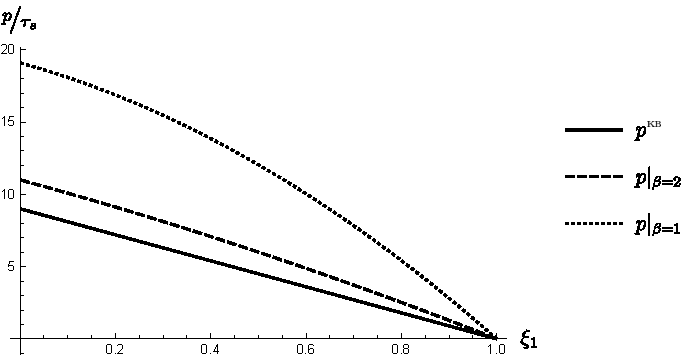
\includegraphics[scale=1.3]{./ch3/pressure}
  }
  \caption{Эпюры давления для случая сферического слоя}
  \label{fig:ch3/sec3/pressure}
\end{figure}

Используя то, что $\alpha(t) = h(t) / \left(\mathcal{R}_0 - h(t) \right)$, где $\mathcal{R}_0$ -- радиус внешней сферы и $h(t) = V(t_*-t)$, можно установить зависимость между временем и стадией прессования:
\begin{equation}
  t_* - t \sim \frac{\mathcal{R}_0}{V} \frac{1}{1+\text{Eu}^{\nicefrac{1}{\beta}}}
\end{equation}
